\documentclass{cup-pan}
\usepackage[utf8]{inputenc}
\usepackage{blindtext}

\renewcommand{\figurename}{Figura.}
\renewcommand{\tablename}{Tabla.}


\title{Implementación de la tesis: \\``Multiple Sequence Alignment using Particle Swarm Optimization''}

\author[1]{Vicente Machaca Arceda}
%\author[2]{Author Two}
%\author[3]{Author Three}
%\author[2]{Author Four}

\affil[1]{Universidad Nacional de San Agustín de Arequipa. Email: \url{vicente.machaca.a@gmail.com}}
%\affil[2]{Department Two, Institution Two, Address Two.}
%\affil[3]{Department Three, Institution Three, Address Three.}

%% Corresponding author
\corrauthor{V.E. Machaca Arceda}

%% Abbreviated author list for the running footer
\runningauthor{Machaca et al.}

\addbibresource{refs.bib}

\begin{document}
	
	\maketitle
	
	\begin{abstract}
		Viral subtyping play a major role for the appropriate diagnosis and treatment of illness. Actually, the most used method for viral subtyping relies on BLAST method that look for similar genomes in big data sets on the Web. The major disadvantages is that we need a big data set where to look for, also we expose the privacy sample genome consulted. An alternative emerged with the use of machine learning models that take the viral sample genome and predict the subtyping. Several methods have been proposed for viral subtyping, based on machine learning models, in this study we compared the two most relevant based on k-mer frequency, Kameris proposed by \citet{solis2018open} and Castor-KRFE proposed by \citet{lebatteux2019toward}. Both have the same results when we avoid their dimensionality reduction and feature elimination, but when not, Kameris slightly outperform Castor-KRFE. Moreover, Castor-KRFE could get a small feature vector for $k>5$ (in k-mer).
		
		\keywords{HIV, Polyomavirus, genome, viral subtyping, k-mer, machine learning.}
	\end{abstract}
	
	
	\section{Introducción}
	El area de Bioinformática ha tenido un auge en las ultimas decadas. Por ejemplo, el proyecto: \textit{The Human Genome Project} (HGP) que inicio en 1990 y fue completado el 2003, donde participarón varios paises como EEUU, Reino Unido, Japón, Francia, Alemania, España y China  \citep{hgp2021}; el proyecto tenia como objetivo secuenciar todo el genoma humano, el cual resulto ser una secuencia de aproximadamente 3.2 billones de pares de bases \citep{archibald2018genomics}. En la actualidad exixten diversas areas de investigación como: la prediccón de estructura de proteinas, predicción de la función de una proteina a partir de estructuras de redes de proteinas, descubrimiento de medicamentos, predicción de enfermedades a partir del genoma, analisis de virus, etc. Es tan grande este campo de estudio que incluso se ha dividido en otras areas como \textit{metagenomics}, \textit{proteomics}, \textit{chemical informatics}, etc. 
	
	\subsection{Problema}
	
	Uno de los tantos problemas que existen en bioinformática, es el alineamiento multiple de secuencias. Se puede definir el alineamiento de secuencias como un método que permite determinar el grado de similitud entre dos o más secuencias \citep{xiong2006essential}, además el método puede insertar \textit{gaps} dentro de las secuencias de consulta, con el objetivo de lograr la mayor cantidad de bases alineadas. Por ejemplo, en la Figura \ref{fig:msa}, se muestra el resultado luego de alinear varias secuencias de aminoacidos. Como podemos ver, se ha isertado \textit{gaps} (-) para así maximizar la cantidad de aminoacidos que coinciden en la misma posición. \\
	
	\begin{figure}[h]
		\centering
		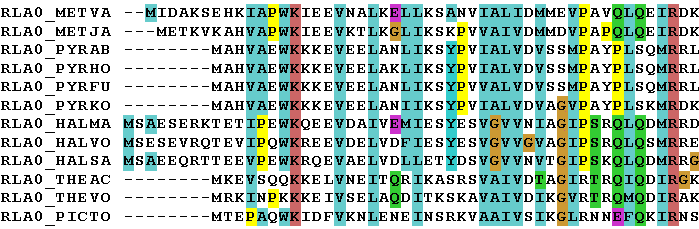
\includegraphics[width=0.8\textwidth]{images/msa}
		\caption{Ejemplo de \textit{Multiple Sequence Alignment} (MSA). El método ha insertado \textit{gaps} (-) en las secuecnias necesarias para maximizar la cantidad de letras (aminoacidos) que concidan en la misma posición.}
		\label{fig:msa}
	\end{figure}

	El alineamiento de secuencias puede dividirse en dos grupos: \textit{pair-wise sequence alignment} (PSA) y \textit{multiple sequence alignment} (MSA) \citep{xiong2006essential}. La diferencia radica en que el primero alinea solo dos secuencias y el segundo puede alinear dos a mas secuencias. Además, el problema de MSA es considerado un problema NP completo \citep{wang1994complexity}. Debido a esto es que se han planteado heuristicas que logran obtener una solución local; el algoritmo mas utilizado es CLUSTAL, fue propuesto por \citet{higgins1988clustal}, este algoritmo ha sido mejorado con CLUSTALV \citep{higgins1992clustal}, CLUSTALW \citep{thompson1994clustal} y CLUSTALX \citep{jeanmougin1998multiple}. Otro algoritmo importante es MUSCLE \citep{edgar2004muscle}. \\
	
	
	El problema de los algoritmos mencionados anteriormente, es que a pesar de ser heurísticas, el tiempo de procesamiento es muy alto. Cada segundo los datos genómicos crecen exponencialmente \citep{archibald2018genomics} y los algoritmos utilizados para buscar información en estas bases de datos, son basados en alineamiento. Entonces, mientras mas crecen los datos, mas lentos se vuelven estos algoritmos \citep{zablocki2009multiple}. 
	
	\subsection{Objetivo}
	
	\citet{zablocki2009multiple}, proponen en su tesis aplicar \textit{Particle Swarm Optimization} (PSO) como alternativa a CLUSTAL para solucionar el problema de MSA.\\

	
	\section{Metodología aplicada}
	
	En esta sección describimos la metodología utilizada por \citet{zablocki2009multiple} para solucionar el problema de MSA utilizando PSO.
	
	\subsection{Representación de las partículas}
	
	Un de los primeros pasos para solucionar un problema utilizando PSO, es la representación de cada particula. \citet{zablocki2009multiple} propone utilizar la posición de cada \textit{gap} como un vector. Por ejemplo en al Figura \ref{fig:pso_1}, tenemos la representación del la partícula \textit{leader} y una partícula cualquiera (ambas representan una posible solución al problema). Ahora en la FIgura  \ref{fig:pso_2}, tenemos otra forma de representar dichas partículas, en este caso solo estamos considerando la posición de cada \textit{gap} insertado. La opción mas facil de controlar es la correspondiente a la Figura \ref{fig:pso_2}. \\
	
	\begin{figure}[h]
		\centering
		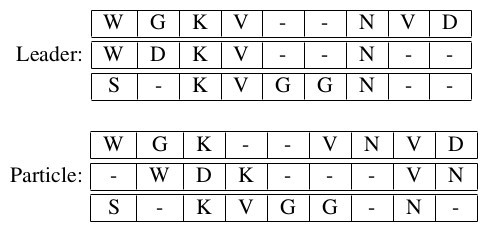
\includegraphics[width=0.6\textwidth]{images/pso_1}
		\caption{Ejemplo de la partícula \textit{leader} y una partícula cualquiera. Ambas representan una posible solución a un problema de alineamiento de 3 secuencias de aminoacidos.}
		\label{fig:pso_1}
	\end{figure}

	\begin{figure}[h]
		\centering
		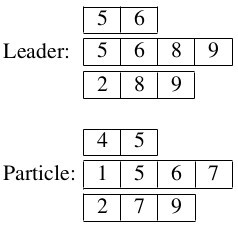
\includegraphics[width=0.3\textwidth]{images/pso_2}
		\caption{Ejemplo de la partícula \textit{leader} y una partícula cualquiera. En este caso solo estamos registrando la posición de cada \textit{gap } insertado.}
		\label{fig:pso_2}
	\end{figure}
	
	\subsection{Movimiento de las partículas}
	Según el algoritmo de PSO, cada partícula debe acercarse al \textit{leader} en cada iteración. Este acercamiento será implementado haciendo un \textit{crossover}. El \textit{crossover} permitirá que la nueva partícula (partícula en movimiento) tenga información de ambas partículas (\textit{leader} y la partícula en movimiento).  \\
	
	Para aplicar un crossover entre dos partículas, debemos calcular primero la distancia entre ellas aplicando la formula de la Ecuación \ref{eq:distance}. Luego debemos calcular el punto de cruce de ambas partículas, para esto aplicamos la formula de la Ecuación \ref{eq:crosspoint}, en este caso $length$ representa la longitud de las secuencias.\\
	
	
	
	\begin{equation}\label{eq:distance}
		distance =  \dfrac{ matchingGaps }{totalGaps} 
	\end{equation}
	
	\begin{equation}\label{eq:crosspoint}
	crossPoint =  rand( 1, distance*length )
	\end{equation}

	Por ejemplo, dada las partículas de la Figura \ref{fig:pso_2} y suponiendo que hemos obtenido un \textit{crossPoint = 5},  utilizando la Ecuación \ref{eq:crosspoint}. La partícula en movimiento se desplazaría y su nueva representación sería el resultado de aplicar un \textit{crossover}. En la Figura \ref{fig:pso_3} mostramos el resultado de aplicar el \textit{crossover}. Para lograr esto, por cada secuencia del leader insertamos sus gaps en la nueva partícula que son menores o iguales al $crossPoint$, luego completamos insertando los \textit{gaps} de la partícula en movimiento que tengan \textit{gaps} mayores al $crossPoint$.
	
	
	
	\begin{figure}[h]
		\centering
		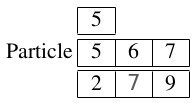
\includegraphics[width=0.24\textwidth]{images/pso_3}
		\caption{Resultado del movimiento de una partícula luego de aplicar \textit{crossover}.}
		\label{fig:pso_3}
	\end{figure}


	\section{Experimentos}
	
	En esta sección detallaremos las bases de datos utilizadas y los parametros del algoritmo PSO para poder replicar los resultados.
	
	\subsection{Bases de datos}
	\citet{zablocki2009multiple} propone un conjunto de 7 bases de datos. S1, S2, S3, S4, S5, S6 y S7 que el construyo a partir de un conjunto de secuencias de ADN. En la Tabla \ref{tab:datasets}, presentamos el \textit{ascension code} de cada secuencia utilizada. Ademas, el autor propuso un conjunto pequeño de secuencias para hacer pruebas rapidas, a este conjunto lo llamo S8. En nuestro caso, al ser una tesis un poco antigua, algunas secuencias ya no estaban disponibles en NCBI, y solo logramos obtener las secuencias de S6, S7 y S8.
	
	\begin{table}[h]
		\caption{Bases de datos utilizados por \citet{zablocki2009multiple}. S1, S2, S3, S4, S5, S6 y S7 es el nombre que el autor definio para cada conjunto de secuencias. La segunda columna representa el \textit{ascension code} de cada secuencia.}
		\begin{tabular}{lp{12cm}}

			\textbf{Dataset} & \textbf{Secuencias} \\
			\hline			
			S1	& HCV2L1A10 HCV2L3A5 HCV2L3C1 HCV2L3C8 HCV2L3D4 HCV2L3E6 HCV2L3A7 HCV2L3A9 HCV2L3B2  HCV2L3B1		\\				
			S2	& HS06674 HS06675 HS06676 HS06677 HS06679 \\
			S3  & TPAHISIN TNIHISIN TNHISIN TMIHISIN TMHISIN THHISIN TFHISIN TEHISIN TCUHISIN TCHISIN TBHISIN TAUHISIN TAHISIN TTHISIN TSHISIN TRHISIN TPYHISIN TPIHISIN TPHISIN TCAHISIN TLHISIN \\
			S4  & HI1U16764 HI1U16766 HI1U16768 HI1U16776 HI1U16778 HI1U16770	HI1U16774	HI1U16772 \\
			S5  & HI1U16765 HI1U16767 HI1U16769 HI1U16771 HI1U16773	HI1U16775 HI1U16777 HI1U16779 \\
			S6  & PP59651 PP59652 PP59653 PP59654 PP59655 PP59656 \\
			S7  & AB023287 AB023286 AB023285 AB023284 AB023283	AB023279 AB023278 AB023276 \\
			\hline 
		\end{tabular}
		
		\label{tab:datasets}
	\end{table}

	\subsection{Parametros}
	
	\section{Resultados}
	

		
	
	\section{Conclusiones}
	
	
	%\blinddocument
	
	%A supplementary material section will always appear before the Reference list. If you're certain that your %submission won't have any supplementary material, you can add the \texttt{nosupp} option to the document %class declaration, i.e. 
	%\begin{quote}
	%\verb|\documentclass[nosupp]{cup-pan}|
	%\end{quote}
	
	\clearpage
	
	\printbibliography
	%\bibliography{refs}
	%\bibliographystyle{apalike}
\end{document}